\section{The Student Software Development Framework}
Over a five year period, a process was created and refined that informed the current framework, which is designed for employing students as software developers for the purpose of developing applications for an academic institution. Following best practices in lean thinking, the framework is constantly being evaluated, redesigned, and optimized each year. Thus, the framework presented in this section represents its current state, but has been generalized as much as possible. It will certainly change as needs of the team and the institution evolve. Figure~\ref{fig:framework} illustrates the framework, including both the summer and regular term, each of which have different structures as described in the remainder of this section. 

\begin{figure}[htbp]
 \centering
 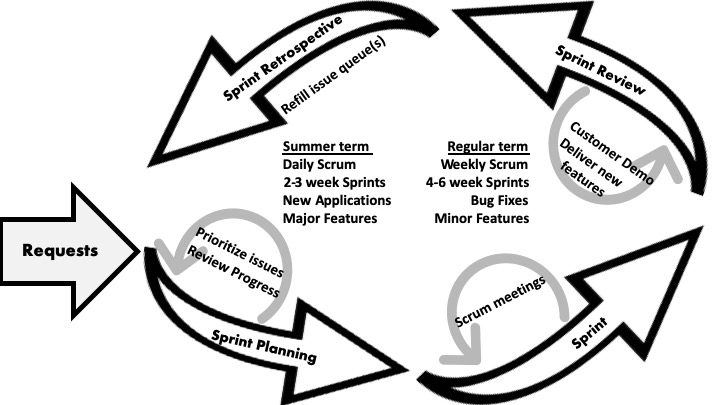
\includegraphics[width=\linewidth]{developmentcycle4.jpg}
 \caption{The Student Software Development Framework}
 \Description{The Student Software Development Framework}
 \label{fig:framework}
\end{figure}

The team of students follow Agile principles \cite{agilemanifesto} using a modified version of Scrum \cite{thescrumguide}. The Scrum methodology dictates that there are three key roles in which all those involved with the development of a software fall under: product owner, Scrum Master, and the development team. The product owner, in relation to the team, is the individual (or group of people) who makes a software request and are the customers who determine the vision and purpose of the software product. Newly added features, fixed bugs, and completed software must be approved and accepted by the product owner before it is considered complete. The Scrum Master is charged with the responsibility of facilitating the development team and communicating the needs of the product owner. The Scrum Master supports and promotes the development team and ensures that the team understands and follows Scrum principles. In our framework, the Scrum Master is not typically a student, unless they have been on the team a significant number of years and can handle the responsibility of guiding the development of the software. Typically, the Scrum Master is a full-time employee of the college (i.e., faculty or staff) who also acts as the team's supervisor. Finally, the development team in this framework consists of undergraduate students who are ``structured and empowered by the organization to organize and manage their own work'' \cite{thescrumguide}. Following Scrum theory provides an iterative, yet incremental approach to cut down on risks and enhance the predictability of the project for the product owner and the development team. 

Scrum also prescribes four events in the software engineering process: sprint planning, the sprint, sprint review, and sprint retrospective. These four events are implemented differently in the framework depending on the term. In the summer, the team follows a more traditional Scrum model with a product backlog and work in progress determined during spring planning, daily Scrum meetings occurring during the sprint, and a Sprint Review and Retrospective happening every two to three weeks before starting the next cycle. In the regular term (i.e., a Fall and Spring term consisting of 16 weeks each), the Scrum time-frame is stretched out due to students working only 10 hours per week instead of 40 hours per week. Daily Scrums become weekly, and Sprints take four to six weeks. Because the regular term is significantly less hours, we often save new systems and major features for the upcoming summer term, while smaller features and bug fixes happen during the regular term. 

This next section will first describe our framework during the summer term, coined the Summer Internship Phase. Then, the following section will describe the framework during the fall and spring terms, coined the Maintenance and Customer Support Phase. 

\subsection{The Summer Internship Phase}
Starting in the summer term, students are hired into the Student Software Development Team (SSDT). Students apply in the previous spring term through an open application process. The students are then hired based on a few metrics, including grades in key classes, such as the CS1 course; their ability to work well with others (based on their interactions with other students in classes, which follow a team-based \cite{2002PairProgramming}, active learning pedagogy \cite{2012Pogil}; and the perceived value they will attain from participating in the program (i.e., the best computer science students are not always selected, as they may not benefit as much from the program), to name a few. 

A typical summer operates much like an internship outside of an academic institution. Students are employed for 40 hours per week for eight to ten weeks, resulting in up to 400 hours of software engineering experience just in the summer alone. During this time, their expectations mirror an internship in many ways, in that they are expected to show up at work on time, be productive throughout the day, and report back to supervisors of their progress. Each summer consists of six to ten students managed by 2 supervisors (one faculty, one staff). The students typically work in pairs as they design interfaces and develop code. 

Early in the summer, students have varying skill levels, but mostly all are untrained on any software engineering principles. All student recruited into the program will have passed the CS1 course, but otherwise, their experience varies. For example, rising seniors will have completed CS2 and maybe a few upper level CS courses, while rising sophomores may have only had CS1. Very rarely will a student have been explicitly trained on software engineering principles, such as Agile methodologies, Model-View-Controller (MVC) or similar frameworks, or large-scale application development.

Contrary to what might seem obvious, the students do not spend a significant amount of time in ``training.'' Instead, we follow a ``just-in-time'' learning principle, where the students are given only as much theory and knowledge about software engineering as is needed to begin the task at hand. For example, one of the first skills students must develop is the ability to work in a version control system, in our case, Git. Students are walked through Git basics, such as how to clone the repository, make commits, and issue pull requests, and then they are given their first issue from the issue queue. Their first issue is often selected very intentionally by the supervisors; for example, finding and fixing a typo in a README of one of the repositories. This gives them the confidence to make a change and issue a pull request to the repository owner, without the fear of breaking any system. 

%%% TODO: MOVE ME this is about the software and how they are obtained; the rest of this section is about the students process. %%%%%%%%%%% The projects are proposed by the campus community (a.k.a. the customer) and are then selected by the faculty member supervising the team. These projects are often tools requested by the customer to help them complete their daily work, and thus, the software becomes an crucial part of the customer’s job. 

A key skill needed and learned by our students very early in the summer internship is the ability to translate customer's needs into usable software (i.e., design). The first step in designing new software is to paper prototype \cite{2003paperPrototype} the software before spending significant hours writing code. This design process consists of many iterations of interfaces on paper; designs are critiqued and modified until there is a group consensus to move forward. Early the beginning of this process, when students are still very new to the idea, the supervising faculty member will act as the "driver," meaning they "click-through" the interface drawn on paper by the students, while those who designed the prototype will move pieces of paper, representing new parts of the interface, to act out its functionality. The first draft typically acts as an eye-opener for the students; the driver will find many flaws and functionalities that their designs are missing. These design mistakes are noted, and the students return to the drawing board to build another version on paper. After multiple iterations, review sessions, and the group approves of the interfaces, the product owner is invited to demo the entire paper prototyped application. Once the product owner's feedback is recorded and taken into account when making the next version. When the interface is finally approved, the paper prototypes are video recorded for later reference (i.e., during coding). 

After paper prototyping is complete, the students review their interfaces and begin to construct the database supporting their prototypes. Again, many of the students have never taken a database design course, requiring more just-in-time training. As a group, they participate in a model building session in which they propose the underlying data structures of the application and the relationships between parts of the model. Multiple design iterations along with guidance from the supervisors lead to the students designing a working database which will support their paper prototypes. One of the key benefits of the students going through this process is they have a much better understanding of the models when they begin implementing their prototypes, reducing confusion about how data is saved and retrieved. 

Having a design in place, plus an understanding of the data model, the students are ready to begin building the application. Students are first given a virtual machine (VM) to develop on, which mirrors the production environment, but also requiring them to learn some basic Linux commands and usage (again, a skill they may not have learned in their courses yet). In pairs, students clone a bare-bones template for the application, with only as much code written for them as is necessary to begin writing code. For example, a main page may be constructed, with minimal content in it, and a basic query to the database to fill it with some dynamic content. From there, the student pairs must replicate the structure of the view and controller into their own interface.

Throughout the process described above, students meet every morning for a daily scrum. It is encouraged and expected that students will have lots of questions early in the summer internship. In fact, most of the just-in-time learning described above happens as a result of the students asking a question. As the summer progresses and the student's capabilities improve, the questions become more technical in nature. In these morning scrums meetings, demonstrations may also occur, as interfaces need reviewed. The students are encouraged to present their incomplete interfaces early, so they can get feedback about components they may impact future code. Lastly, code is often brought up to demonstrate good and bad coding practices, and correct them before the problems become too large to handle, to avoid large amounts of refactoring. 

As the summer progresses, the supervisors take an increasingly hands-off approach, expecting the students to ask each other for help first. This promotes sharing of knowledge among teams, as pairs begin to solve problems that others have already solved (or similar), and know some of the pitfalls to avoid. To maintain organization and visibility about what features each team is working on, we leverage Kanban boards, or Work in Progress (WIP) boards \cite{anderson2010kanban}. Applying the Kanban model in tandem with the Scrum framework aids in managing the overall flow of the project. The Kanban model prioritizes three essential principles: visualize what will be done today, reduce the amount of work that is in progress, and properly manage the flow. Kanban encourages continued cooperation and creates an environment that promotes ongoing learning by describing the optimal team workflow. The blending of Kanban and Scrum is also known as Scrumban \cite{ladas2009scrumban}. Figure \ref{kanban} shows the most recent iteration of our Kanban board (which has changed many times as the team finds ways to improve its usefulness).

\begin{figure}[h]
 \centering
 \label{kanban}
 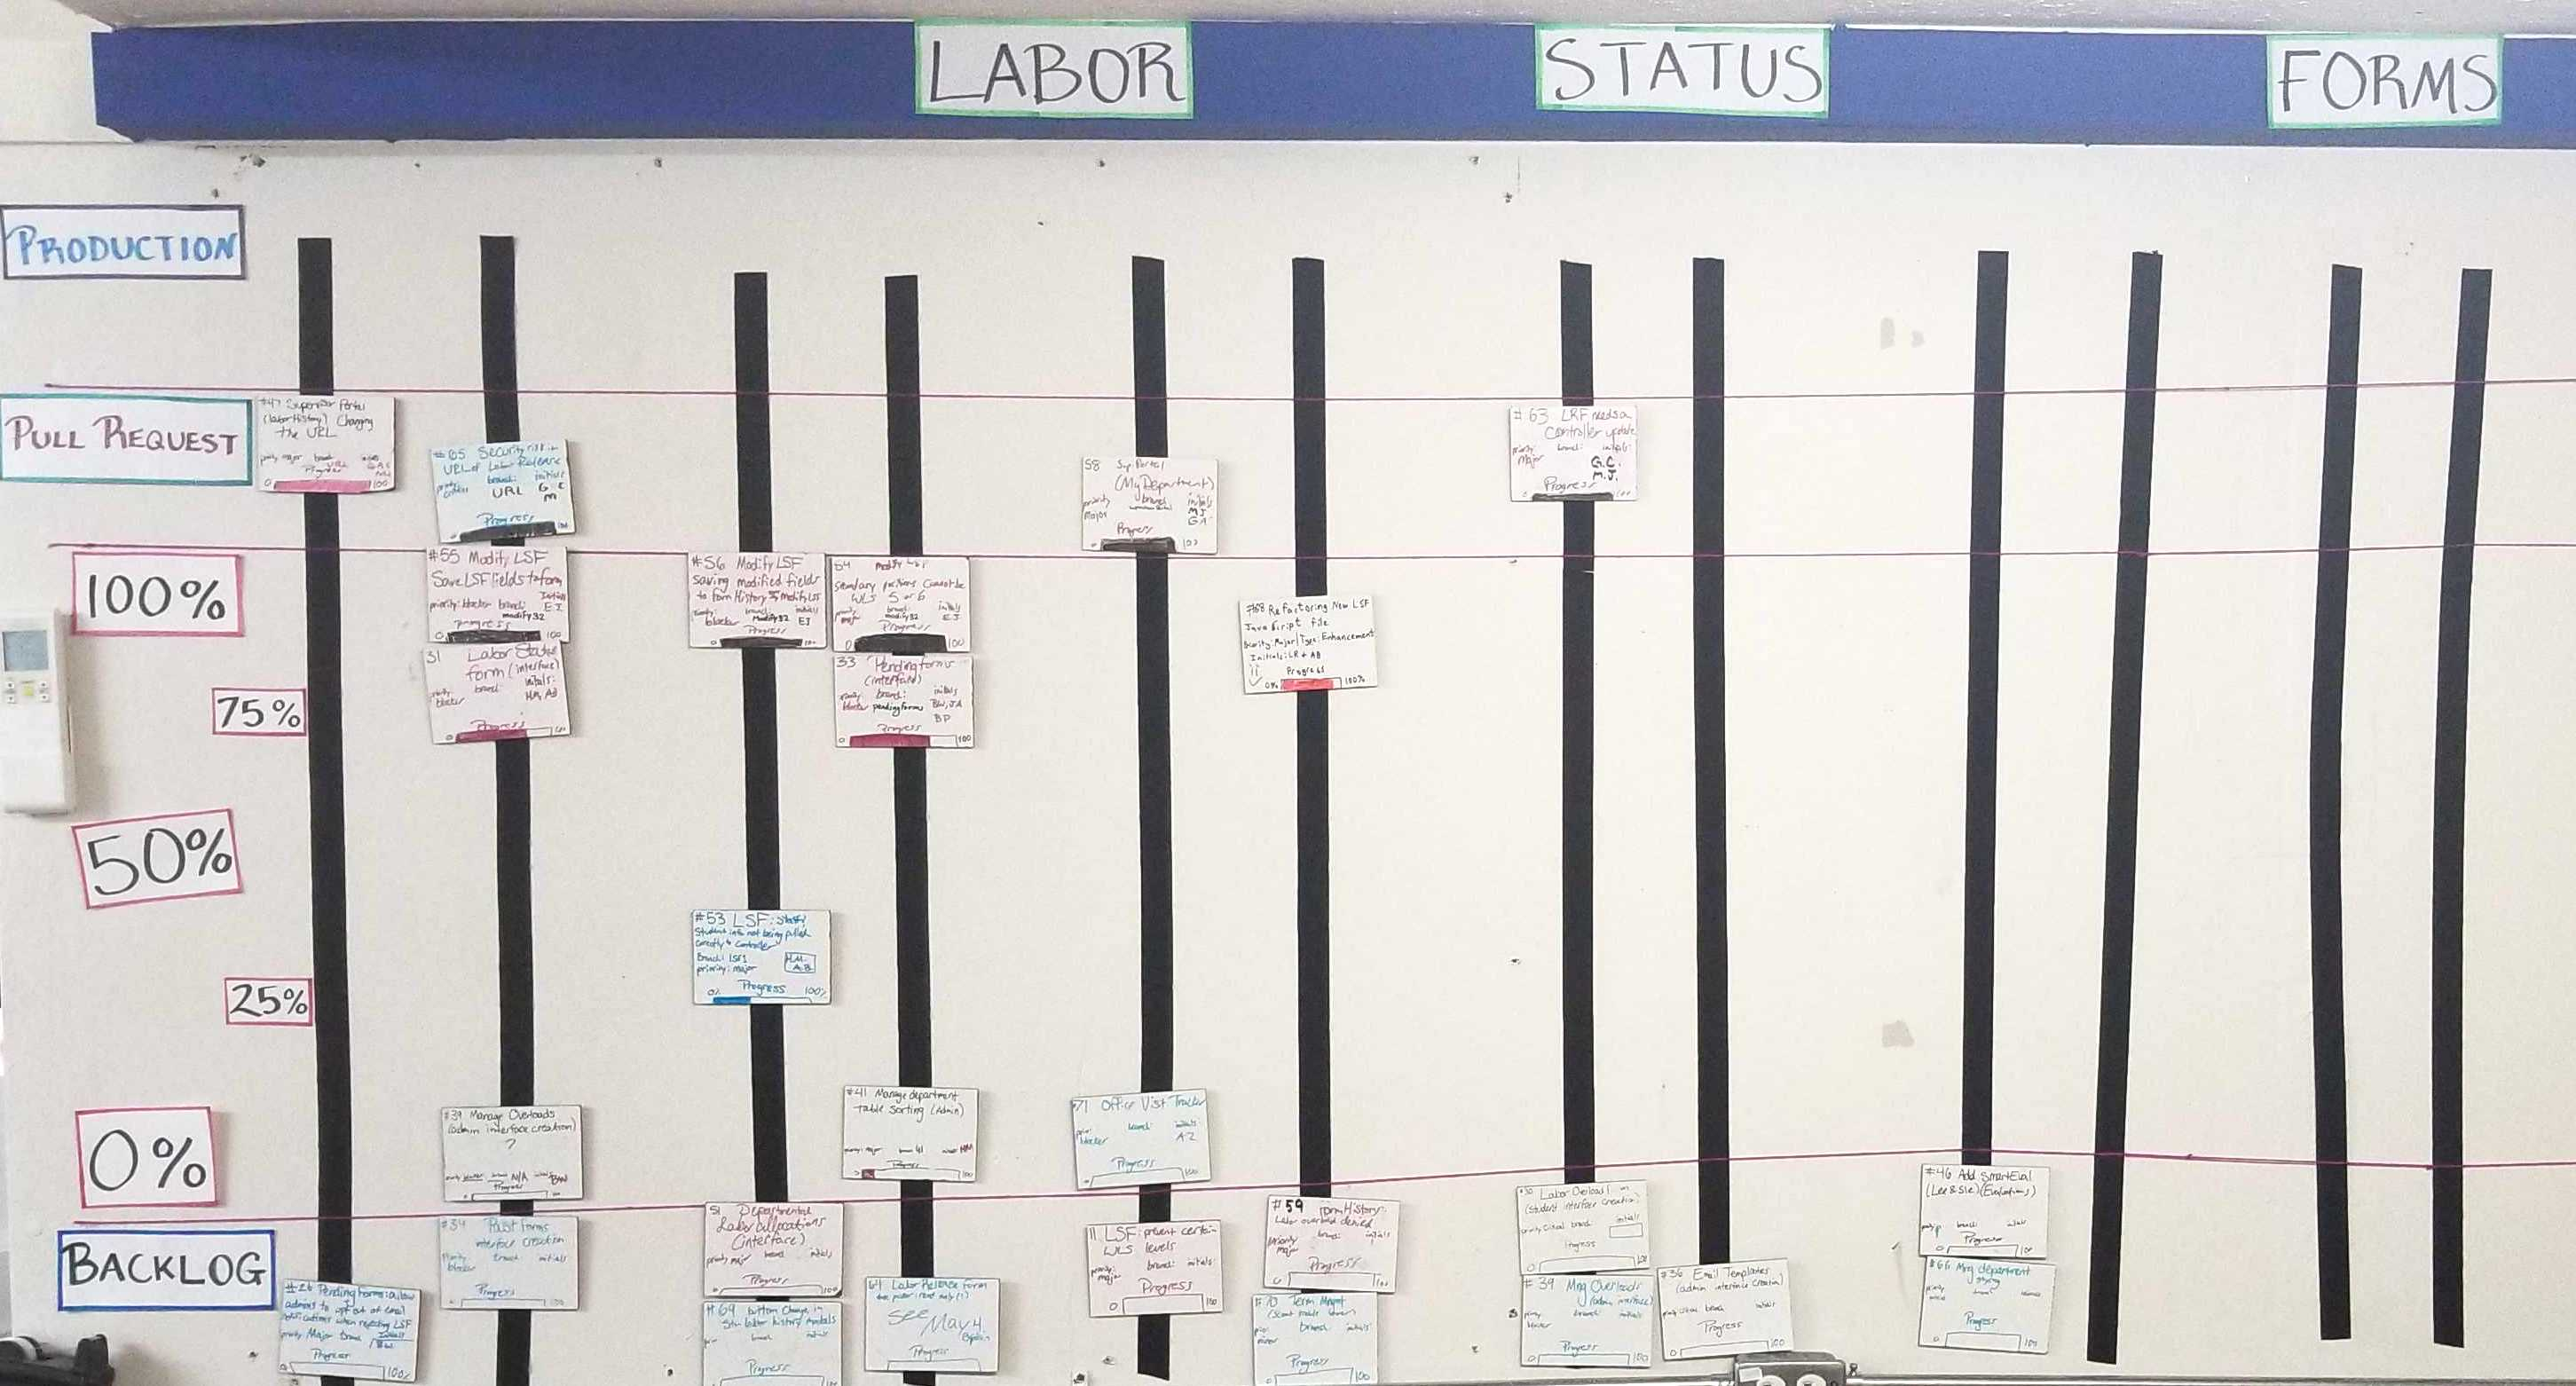
\includegraphics[width=\linewidth]{kanban.jpg}
 \caption{Kanban board for organizing team progress}
 \Description{Kanban board for organizing team progress}
\end{figure}

Another important tactic in promoting the sharing of knowledge involves rotating teams. The team lead and supervising faculty member conduct a meeting a few weeks into the summer term to evaluate each pair's performance. They evaluate each developer's strengths and weaknesses, then redistribute the teams. Typically one developer stays on the interface they were currently working on developing, and gain a new partner who is new to the interface. Shuffling the pairs helps students be flexible, learn to collaborate with others, and most importantly, reveals the importance of well-documented code and following coding standards adopted by the team. It also encourages the students to be able to explain their progress, clearly articulate their goals, and know exactly what their code does as they explain it to their new partner. 

As interfaces get close to complete, the pair is expected to conduct a usability test \cite{usabilitytesting}. The pair will run the usability test first with another team who has not used their interface. They provide them with a set of tasks or scenarios to complete, and observe the user. Usability tests show students faults they may not have seen in their interfaces. For example, as they are developing, they will commonly only test the expected use case. The usability test might reveal that there is another set of operations that the user can do which causes a crash. After fixing these new bugs or improvements, they will conduct another usability test, typically with the supervisors as the driver. It is expected that there will be less (but rarely none) new bugs or usability problems to fix. A third (or more) usability test is then conducted with the product owner, to get their final approval of the implementation.  

Ideally, by the end of summer, the product is delivered to the customer fully implemented. As this is not always the case, constant communication with the product owner as well as clearly setting expectations very early alleviate issues with surprises about delays in deployment. Any features that aren't completed in the summer term become issues for the team during the regular term, after critical bugs are resolved (more on this in the next section). 

% BRI - Talk about how we use Agile methodologies, scrum, and kanban for managing software projects. Take a (good) picture of the wall you just created for LSF as an example of Kanban.

\subsection{The Maintenance and Customer Support Phase}
As the Fall term begins, the team shifts from working 40 hours to 10 hours per week, as the students are now also responsible for attending classes and other academic responsibilities. As expected, the productivity of the students shifts dramatically between summer and the regular terms. The framework takes this into consideration. Whereas summer terms focus heavily on designing new, major features or entire software systems, the regular term focuses more on maintaining existing software and responding to customer needs (e.g., bug fixes or small feature requests). The expectation is that the regular term provides students with the valuable experience of having to maintain their software after deployment, a skill rarely taught in software engineering courses after projects are ``completed'' and delivered to customers.

Students meet with the supervisors at the beginning of the Fall term to schedule their hours around their courses and other academic responsibilities, with the goal of ensuring no student is working alone for extended periods of time. Students who work alone for too much of their time develop bad coding habits without their code being reviewed frequently, leading to wasted effort as the code they create doesn't make it to the final product. Similarly, students working alone make bad design and usability choices as they implement, leading to useless software. Lastly, if the student gets stuck on a problem, there is no one there to brainstorm solutions with them. The supervisor, in our case a faculty also teaching courses, isn't as available to assist the students as quickly, meaning they must rely on each other to get unstuck moreso than during the summer. It is crucial that students work with other students to fix bugs and solve problems in order to maintain steady progress in development.

Work duties are mostly determined by the users as they encounter bugs, and the product owner, as they start thinking of new features they want in their software. Customers report bugs or new feature requests via email to the supervisors, who evaluate the priority and difficulty of the issue. The issue is then added to the issue queue for that application. If the issue is urgent (e.g., causing crashes or rendering an interface unusable), the issue is taken by the first student that is available (i.e., the next one to come to work). In some cases, the bug warrants one or more of the supervisors to work on the issue immediately. For non-critical issues, the issue is discussed in the weekly scrum meeting and added to a team's work in progress, or left in the issue queue if it's not considered the most pressing issue for that week. 

% Back to the kanban board...
Similar to summer, the Kanban board is instrumental to keeping the team organized and aware of each others' work, particularly since the students' schedules become more spread out. Students check the Kanban wall for new issues, claim them, and keep record of their progress on the wall. This flow helps developers visualize their progress and estimate their time, which is essential given they only have 10 hours per week to work. When the issue is resolved and tested by multiple student developers, a pull request is issued. Pull requests are reviewed by the supervisors, and returned if there are errors or standards not followed. An accepted pull request must pass our guidelines for coding structure, naming conventions, security, and best practices. The supervisors are responsible for the last mile; integrating the feature into the production environment. Sometimes bugs are found during integration, which are pushed back down into the repository, requiring all developers to pull in these changes (as well as the new feature itself) to synchronize the everyone's local environments. 

\section{The Software}
% Quick paragraph... improve?
This section begins by describing the process for selecting new requests for software, followed by a brief summary of the software that has been generated by the SSDT. Lastly, two examples of applications built by the SSDT are presented.

\subsection{Selecting Software Requests}
The team receives software requests from departments and offices at the institution who are aware of the Student Software Development Team and think we can help them. In some cases, the department needs to replace old or inadequate software they already own. In other cases, they are still relying on inefficient paper processes that could easily be replaced with a software solution. It is also not unlikely for team members to reach out to departments and inquire about their needs. When a software request is received, the team reviews the request and determines which projects are feasible and which lie outside of the mission of the team. Selected projects go into a backlog to be considered in the upcoming summer. A number of factors determine which systems we will implement, including the request's urgency, value to the institution, and the expected effort required to complete the project. All of these factors are weighed in order to select the request that best fits our capabilities and current capacity.

% % CUT?
% \subsection{Software Engineering Principles}
% After a software request is selected, the summer term starts with the team following the principles and values described in the Agile Manifesto to begin building the software solution. The Manifesto does not provide concrete or descriptive instructions on how to develop software, but instead provides fundamental information to be considered throughout the entirety of the software development from project initiation to project close. Agile software development prioritizes interactions within the software team as well as with the customer, and encourages software processes that are receptive to change while still delivering quality software \cite{agilemanifesto}. % How are we using it?

% % CUT The hybrid of Scrum used by the team also intertwines the Kanban model into its practices.
% Scrum methodology is a subgroup of the Agile project management framework that articulates more details and specifications on how to employ the principles in the Manifesto within the team's software development practices with ``the goal of delivering new software capability every 2-4 weeks'' \cite{thescrumguide}. [BRIACHECKTHIS] Scrum is the most popular agile methodology; ``According to the 12th annual State of Agile report, 70 percent of software teams use Scrum or a Scrum hybrid'' \cite{}. 



% Cut? The four Scrum events complemented with Kanban references these events as ``flow-based events'' to acknowledge the importance of managing the teams workflow during these events. The Summer term, when students work for 40 hours a week, is when the team can execute these events to the full extent as the team is able to convene in a way that is comparable to that of a software team that works full-time year round. The Sprint Planning begins when the team decides which customer request will be the central focus for that year. This event is used to outline the work that will be performed during the Sprint. The Development Team uses this time to forecast the range of capabilities that will be developed during the Sprint and to also set the Sprint Goal. The Sprint Goal for the SSDT is to have a beta product available by the end of the Sprint. When a software is released in beta, the majority of the software requirements have been met, however,there may be small issues that have yet to be addressed. By releasing beta versions of products, the SSDT and the Product Owner are able to observe most of the functionality of the software that has already and also test for inconsistencies. Close communication with the customers is crucial to the development of the software; staff's needs may change, college policies may update, and staff may move on to jobs elsewhere. As needs change, SSDT can adapt to and account for them.

% Repeat of above words
% \paragraph{Sprint Planning \& Paper Prototyping}
% Sprint Planning begins with analyzing the current processes that the Product Owner is utilizing*. Asking questions such as, What does the current software that is used to solve their problem look like? How does it work? Are they using any software? Where is the data that needs to be tracked currently being stored? What forms have to be filled out and which people have the authority to approve this process before it is considered to be done and put into action. For instance, if the Product Owner was requesting a software that allows students to add and remove courses to their schedules. The SSDT would need to know how students are currently able to do this task and then make sure to add it to the requirements of the software that is being built. During the SSDT's most recent Sprint, the request that was chosen involved doing an entire refactoring of a live* software.

% In order to get a better idea of the functionality of the new software should be implemented, the Development Team begins by going through multiple iterations of paper prototypes. Paper prototyping is a prototyping method in which paper is used to simulate a computer or web application. A paper prototype should hold all of the functionality that the finished user interface of the application will have; from navigation bars, drop down menus, and headers to button clicks and items that will hover on the interface. A person should be able to ``click-through'' the website via the paper prototype. To start this process, screenshots of the old software's interfaces were taken and printed out. Next these interfaces are critiqued* and analyzed to decide which parts are to be kept for the refactoring, which parts will need to be reworked, and which parts will need to be discarded altogether. The purpose of this part of the paper prototyping process is to become familiar with the current software so that the team can adequately build a better software. The team looks for things* such as bugs, broken links, slow page loading, poor user design, etc. and makes a note of these issue to ensure that they are addressed in the new software. After the individual interfaces of the previous software have been discussed and analyzed, the team divides the different interfaces into two categories: Main and Administrative. Main interfaces are the web pages that all users of the application will be able to see whilst Administrative web pages will only be accessed by system administrators, such as BC staff and SSDT's supervisor.

% Next the team breaks down the interfaces into issues in which the team will tackle* in pairs. The pair of developers then begins to design the interface that they had chosen from the interfaces that needed to be refactored. Each time a pair from the team believes that they have successfully created a valid* paper prototype, it is then tested for usability. Paper prototyping testing occurs* in the same way that a fully functional software would be tested, the person testing the paper interface will treat it as such. The tester will ``click'' on different components of the interface and the designers will physically move parts and replace parts of the paper interface in order to replicate how the real software would respond. The pair who designed the interface will take notes as the tester navigates their paper web page and when the test is complete, they use these notes to redesign and the process is repeated. Paper prototyping is done because ``bug'' and inefficiencies are easier to fix when no coding has been done yet and one can go through many iterations without having to actually having to troubleshoot actual code. The SSDT repeats this process of designing, testing, and re-designing until the entire team is satisfied with the final iteration. After all interfaces have been drafted and prototyped, the process of building the application begins and the team commences the Sprint.

%TODO Do we want to go into Flask, Peewee, Jinja, etc. or keep it generic? 

\subsection{Software Built by the Student Software Development Team}
The vast majority of the applications created by the SSDT are browser-based web applications. The SSDT follows an MVC architectural model to structure all of the applications. The team uses Flask, a web framework that uses Python as a back-end language (i.e., the controller), designed to make the start-up of a web application fast and easy. Coupled with two Python libraries, Jinja for template rendering (i.e., the view) and Peewee for database abstraction and integration (i.e, the model), the team has all the tools needed to begin building web applications. Since most of our applications are intended to be tools for doing work (as opposed to web sites for selling products or advertising services), we leverage Bootstrap for webpage styling and simplifying the implementation of the front-end of the application, particularly related to mobile-readiness. 

In the five years since the creation of the SSDT, we have started twelve software systems. Of those twelve, three are retired and one is not maintained by our team any longer. The remaining eight applications are regularly maintained by the SSDT. Communications with the product owners occur at a minimum twice a year, where new features are proposed by them as they discover more ways in which the software can support their work. Each system was initially designed to serve a specific need within the product owner's department. For brevity's sake, we will describe two of these applications that are of relevance to many academic institutions.

\subsubsection{The Chemical Inventory System}
One responsibility of the Environmental Health and Safety department is to track and control the movement of hazardous chemicals on campus. Chemicals must be stored in a special bunker, and certain regulations exist for certain chemicals. For example, some hazardous chemicals cannot be stored above specific quantities, depending on which floor the chemical is on. 

The institution was managing the chemical inventory through dated software which was slated for retirement. The department needed a new solution, but was not given an adequate budget to purchase existing solutions that served their exact needs. The SSDT was approached to implement a solution which solved the needs specifically for the department. 

The SSDT created a web-based application which allowed the department to track the purchase, movement, and disposal of all chemicals on campus. The application had the added benefit of providing controlled access to interested individuals, such as chemistry faculty, to be able to view the current stock of each chemical, as well as see where they are currently stored and the age of the chemical. The system was extended further to include the ability to quickly generate a report for a building (in case of emergencies, such as a fire), as well as document the disposal of chemicals and track the history of a chemical as it moved to different places. In all, the software made the campus a safer place to work, improved visibility about the chemical inventory, and resolved issues of missing chemicals and data inconsistencies from years of use by the prior tool.


\subsubsection{Course Administration and Scheduling (CAS)}
The Course Administration and Scheduling (CAS) application was first requested by the Registrar's Office at our institution. Prior to the system, the Registrar's Office would send an email out to all of the department chairs at the institution requesting the schedule for upcoming terms. Included in the schedule were the course title, prefix and number, the faculty member(s) who would teach the class, the number of students who could take it, which room on campus was needed, if any, and the time of the course, to name a few. Department chairs would then respond to the email with their drafted schedule. This data would get get aggregated into a single spreadsheet by the Registrar, then emailed back out to the department chairs for review. This process would repeat for multiple weeks as department chairs resolved conflicts in scheduling (e.g., ensuring required courses from other departments not overlapping), each week requiring the Registrar to update the spreadsheet. To further complicate the process, one additional chair would need to approve all courses for their division (i.e., multiple departments), and some courses are not as straightforward as others (e.g., special topics courses, cross-listed courses, team-teaching situations, prerequisites, co-requisites, to name a few). 

This process was error prone and inefficient for the Registrar's Office staff as well as the department chairs. The SSDT was approached to develop a software solution that would improve the situation for everyone. 

The SSDT developed CAS, a web application that allowed department chairs to enter in all of the course information for their department. Each department chair had access to edit their own department, and could view the schedule of all departments as the schedule was being constructed. The Registrar's Office staff had access to edit all courses in all departments (i.e., administrator access). The application provided data validation tools to ensure only valid inputs were allowed (e.g., course numbers and titles matched the institution's course catalog), as well as the ability to indicate all of the non-standard courses, as mentioned above. The Registrar was given the ability to lock the term at a specific date, at which point no additional changes were allowed in the system. The full list of courses was then exported from our application and imported into the official schedule for that term. 

The application was well-received, particularly by the Registrar's Office, who was no longer spending significant hours managing spreadsheets via email. The application has also survived multiple staffing changes, including a new Registrar and two new Assistant Registrars (who interacted with the software the most). In each case, the new staff member was able to learn the software quickly and integrated it into their workflow. The Registrar's Office has also requested new features and changes to existing features to be integrated into the system since its creation. For example, a matching algorithm was added to facilitate a more unbiased approach to assigning rooms to classes, particularly in popular rooms where multiple faculty would lobby to the Registrar to be given that room. All faculty are now able to enter their preferences for rooms, and the system will attempt to assign everyone a room based on those preferences, without creating any room conflicts. 

The CAS application started as a simple scheduling tool, and has evolved over the last four years into a much larger application for managing multiple aspects of course scheduling, empowering faculty to have more voice in their room placement, and improving visibility of the larger schedule to the entire faculty and staff.

% CUT During the Sprint, the team convenes everyday in the morning in order to touch base with each of the pairs within the team and get an idea of their progress. During the Scrum meeting, the smaller teams tell what the have accomplished since the last meeting, what they will begin to work on next and what they will be completing before the next Scrum meeting, and where they are stuck or if any obstacles got in the way of completing their previous work. Scrum meeting (also called the Daily Stand-Up) is for quick communication purposes and should take no longer than 15 minutes. Sometimes small demos are done during the Scrum meeting in order to get the entire teams' input on certain features before proceeding. The programmers are expected to do a ``DDS'' in a team collaboration application called Slack, DDS stands for Did, Doing, and Stuck. During the Academic Year, these updates serve to compensate the lack of daily Scrum meetings; all students are not available at the same time while classes are in session. Team leaders examine the DDS reports to ensure progress is steady as well as evaluate who needs guidance. These updates also aid in communication between team members if they happen to not see each other. Instead of having a daily Scrum, we instead have a weekly Labor Meeting in which we present and evaluate the team's progress and state in production.

% \paragraph{SPRINT REVIEW}
% The Sprint Review's purpose is to inspect the amount of work that was completed during the Sprint and measure the amount of work needs to be completed for the next Sprint. The SSDT uses a version control application called GitHub that allows them to edit parts of the software using a copy of the application in their own environment without interfering with the main program. When the Sprint is completed, the parts of the application that were successfully finalized during the Sprint are merged into the main program. This will allow the team to then create another copy of the main program that now has the new changes and fixes to include in the next Sprint. After the Sprint is completed, the team does an overall demonstration to present the work that they have completed during the Sprint. After the team demonstration, the Product Owner is brought in so that the team can present the work that has been completed so far. It is important that the Product Owner also participates in the Review; their job is to make sure the work so far meets their criteria and requirements. They also have the authority to reject part of the application, suggest modifications to what has been built, or request a feature be added to the application. The feedback from the Product Owner during this stage is essential as it defines new criteria for the next wave of implementation.

% The Review is also used to help set goals for the next iteration. The team holds another meeting to discuss what issues and features were supposed to be completed by the end of the Sprint, but did not. Of those issues, how close are they to being completed and what is a realistic goal that be set for completion in the next Sprint. The SSDT will also review the work that was added during the Sprint or the work was removed. This will give the team insights about what goals may have been too ambitious for the Sprint deadline and what goals could have had more tasks added to them. The Review helps the SSDT to transparently assess the capabilities of the team.

% \paragraph{SPRINT RETROSPECTIVE}
% This is the final meeting after the Sprint in which the team discusses the overall process and performance of the Sprint. The Sprint Retrospective provides an opportunity for the SSDT and the Scrum Master to strategize ways to improve their methods and approaches for the next Sprint. The objective of this part of the Scrum process is not to focus so much on the work itself but to evaluate the processes of the team. During the meeting, the team finds what activities worked well and should continue to be used in the future, what went wrong during the Sprint, and what could be improved for the next iteration. This meeting is not, however, designed to assess the performance of an individual or to penalize anyone for any shortcomings. The intention of the Retrospective is to gather information about ways to improve the next Sprint. During this discussion, the team openly explores the difficulties and challenges faced during implementation. The team's strengths and triumphs are examined alongside the setbacks to better prepare for these challenges in the future.

% \subsubsection{The Academic Term} 
% The Fall and Spring terms are both comprised 16 weeks* where most students work at least 10 hours a week. Upperclassmen students can work up to 15 hours a week, if permissible. In addition to class scheduling occupying the students' weekly routines, the weekly labor restrictions follow the guidelines established by the labor program at the institution.


% "MOVE ME" ``The SDDT at our institution was established over four years ago with the Student Software Development Initiative by a Computer Science faculty member.''

% "DONT THINK WE NEED THIS" ``Students learn real-world work skills such as time management, and responsibility. Some students move up into positions of leadership and build those skills. Between classes, extracurriculars, and secondary labor positions, SSDT's staff dedicate time to their labor hours.''